\documentclass[11pt]{beamer}
\usepackage{verbatim}
\usepackage{amsmath}
\usepackage{amsthm}
\usepackage{graphics}
\usepackage{multicol}
\usepackage{color}
\usepackage{stmaryrd}\usefonttheme[onlymath]{serif}

\title{Progess Report 3}
\date{\today}
\author{Xie Li}
\begin{document}
\maketitle

\begin{frame}\frametitle{Overview of the Progress}
\begin{itemize}

\item Introduction to \textsc{KLEE} and static analyzer of \textsc{AbsInt}

\item A summary of the tools: capabilities and algorithms.

\item A survey paper.


\item Currently working on designing data structures for later development.
\end{itemize}

\end{frame}

\begin{frame}\frametitle{Tool Survey: \textsc{KLEE}}

\textbf{Usage: }

\texttt{llvm-gcc --emit-llvm -c code.c -o code.bc}


\texttt{klee --max-time 2 --sym-args 1 10 10--sym-files 2 2000 --max-fail 1 code.bc}

\textbf{Algorithm and Techniques:}

\begin{itemize}
\item Symbolic Execution.\\
\item Maintaining of path condition of the path.

\item Classify dangerous operation and when bug identified use SMT solver to find concrete value.
\end{itemize}

\textbf{Application:}

KLEE was applied and reach a coverage of 81\% of GNU \texttt{Coreutil}. It found totally 10 errors and even some bugs in heavily-tested code.
\end{frame}

\begin{frame}\frametitle{Tool Survey: \textsc{Astree} of AbsInt}
\textbf{Toolset:}
Check C code for runtime error: \textsc{Astree}.

Check code guideline: \textsc{RuleChecker}.

Compiling: \textsc{CompCert}.

Check Stack usage: \textsc{StackAnalyzer} 
.

Analyze execution time: \textsc{aiT, TimeWeaver}.

\end{frame}

\begin{frame}\frametitle{Tool Survey: \textsc{Astree}}
\textsc{AbsInt} focuses on non-functional program errors.

\textbf{Capability:}
Check
\begin{itemize}
\item Division by zero
\item Out-of-bounds array indexing.
\item erroreous pointer manipulation and dereferencing
\item interger and floating-point arithmetic overflow
\item read uninitialized variables
\item data races
\item inconsistent locking
\item violation of user-given assertions
\item unreachable code
\end{itemize}

\end{frame}
\begin{frame}
\frametitle{Summary of Tools}
\begin{itemize}
\item 
\textsc{CBMC}: verifies memory safety (array bounds and safte use of pointers), check for exceptions. Algorithm used: bounded model checking. 
\item 
\textsc{NuSMV}: a symbolic model checker utilizing BDD library and able to model and check.

\item 
\textsc{CPAChecker}: a static analyzing tool capable of  doing data-flow analysis and automatic testing. Algorithm used: CPA algorithm which integrate several static analysis algorithm based on abstract intepretation, symbolic execution for automatic testing  and CEGAR loop for refining.

\item 
\textsc{Infer}: A static analysis tool used mainly for finding bugs for programs that manipulating heaps and memory. Algorithm: inference of separation logic and invariant synthesis using shape analysis, incorrectness logic inference.

\item 
\textsc{KLEE}: A testing tool based on llvm use symbolic execution for automatic testing.

\item 
\textsc{Astree}: A static analyzer detecting runtime error. Algorithm: Abstract intepretation.


\end{itemize}


\end{frame}

\begin{frame}\frametitle{Functionalities of Tools}
\begin{tabular}{c|c|c|c|c|c|c|c}
Toolname & AI & CE & BMC & SMC & SE & Conc & SA\\
\hline 
\textsc{CBMC} & & $\times$ & $\times$ & &$\times$& &\\
\textsc{CPAChecker} & $\times$ & $\times$ & $\times$(dep.) & & $\times$ & & $\times$\\
\textsc{Infer} & & & & & & &$\times$\\
\textsc{KLEE} & & & & $\times$ & &\\
\textsc{Astree} &$\times$& & & $\times$ & &$\times$\\ 


\end{tabular}
\end{frame}

\begin{frame}\frametitle{Survey Paper}
A Survey of Automated Techniques for
Formal Software Verification
\begin{center}
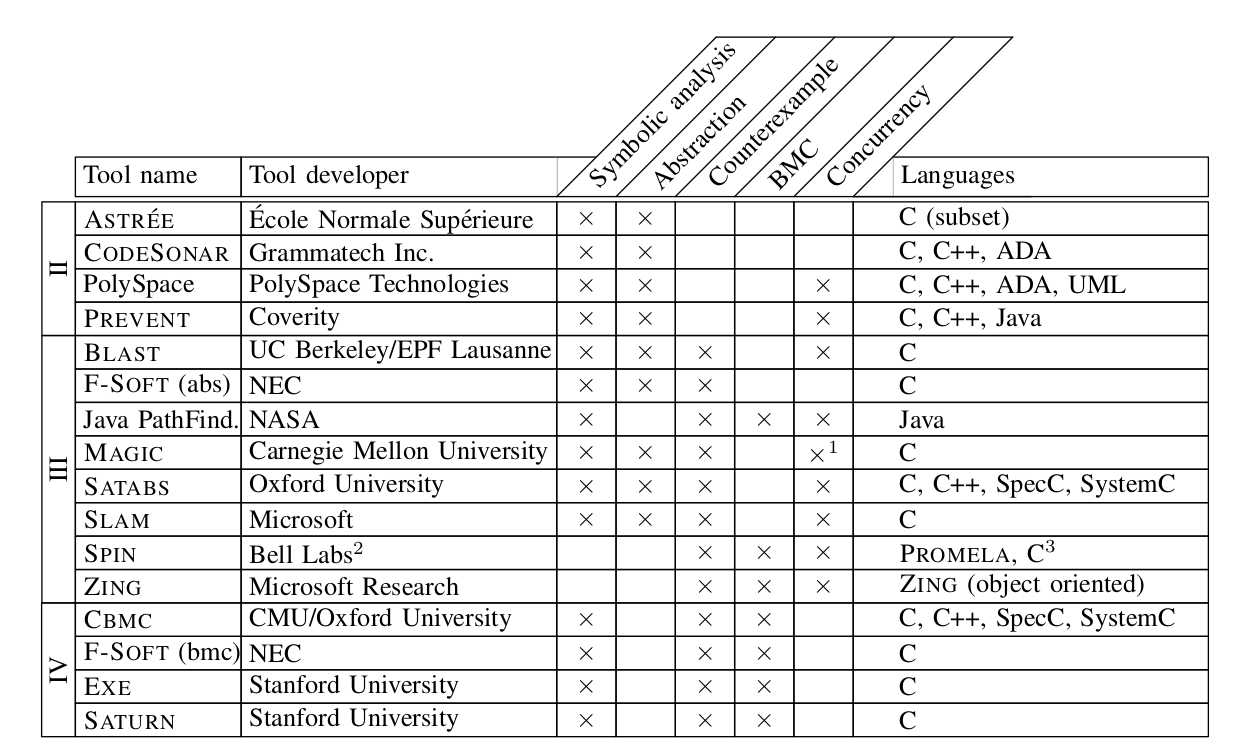
\includegraphics[scale=0.24]{table.png}
\end{center}
\end{frame}
\begin{frame}
\begin{center}
LLVM Pass \& LLVM C++ API


\end{center}
Compiling of llvm pass:

\texttt{
clang `llvm-config --cxxflags` -Wl,-znodelete -fno-rtti -fPIC -shared [Passname].cpp -o [Passname].so `llvm-config --ldflags`
}
\texttt{opt -load ./[Passname].so -[Pass] [filename].ll}

Compiling of llvm api:

\texttt{ c++ IRReaderTest.cpp `llvm-config --cxxflags --ldflags --libs core` -o a}
\end{frame}

\begin{frame}\frametitle{Later Work}
\begin{itemize}
\item Design of the abstract data structure.

\item Building the gap between LLVM data structure and our own data structure.
\end{itemize}
\end{frame}

\end{document}